As it was mentionned in sec. \ref{sec:QSH}, the QSH effect requiers strong spin-orbit coupling to occur. Kane and Mele initially proposed that the effect could be realised in graphene but the spin-orbit coupling of carbon is too weak \cite{cayssol_topological_2021}. The first observed topological insulator with QSH effect is a mercury telluride heterostructure consisting of a staking of thin \ch{HgTe} layers between \ch{Hg_xCd_{1-x}Te} \cite{kane_this_2011}. The Band structure of \ch{HgTe} and \ch{Hg_xCd_{1-x}Te} both contain a $\Gamma_6$ and $\Gamma_8$ band \cite{bernevig_topological_2013}. While the $\Gamma_6$ band is $s$-type, the $\Gamma_8$ band is $p$-type. A $s$-type (resp. $p$-type) is formed with the hybridization of $s$ (resp. $p$) orbitals with $0$ (resp. $1$) angular momentum quantum number \cite{girvin_modern_2019}. Adding spin leads to $1/2$ and $3/2$ respective total angular momentum quantum number for $\Gamma_6$ and $\Gamma_8$ bands \cite{bernevig_topological_2013}. 

If the thickness of the \ch{HgTe} layers is right, a spin Hall effect arises. \ch{Hg_xCd_{1-x}Te}

The signature of the appearence of a topologial phase with variation of the thickness is the band inversion \cite{bansil_colloquium_2016}. 

\begin{figure}[h!]
    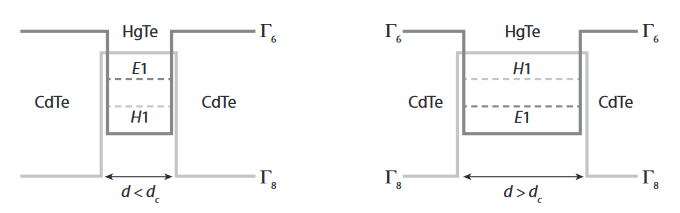
\includegraphics{sections/visuel/Hg}
    \caption{\cite{bernevig_topological_2013}}
\end{figure}